\documentclass{beamer}

\mode<presentation> {
	
	% The Beamer class comes with a number of default slide themes
	% which change the colors and layouts of slides. Below this is a list
	% of all the themes, uncomment each in turn to see what they look like.
	
	%\usetheme{default}
	%\usetheme{AnnArbor}
	%\usetheme{Antibes}
	%\usetheme{Bergen}
	%\usetheme{Berkeley}
	%\usetheme{Berlin}
	%\usetheme{Boadilla}
	%\usetheme{CambridgeUS}
	%\usetheme{Copenhagen}
	%\usetheme{Darmstadt}
	%\usetheme{Dresden}
	%\usetheme{Frankfurt}
	%\usetheme{Goettingen}
	%\usetheme{Hannover}
	%\usetheme{Ilmenau}
	%\usetheme{JuanLesPins}
	%\usetheme{Luebeck}
	\usetheme{Madrid}
	%\usetheme{Malmoe}
	%\usetheme{Marburg}
	%\usetheme{Montpellier}
	%\usetheme{PaloAlto}
	%\usetheme{Pittsburgh}
	%\usetheme{Rochester}
	%\usetheme{Singapore}
	%\usetheme{Szeged}
	%\usetheme{Warsaw}
	
	% As well as themes, the Beamer class has a number of color themes
	% for any slide theme. Uncomment each of these in turn to see how it
	% changes the colors of your current slide theme.
	
	%\usecolortheme{albatross}
	%\usecolortheme{beaver}
	%\usecolortheme{beetle}
	%\usecolortheme{crane}
	%\usecolortheme{dolphin}
	%\usecolortheme{dove}
	%\usecolortheme{fly}
	%\usecolortheme{lily}
	%\usecolortheme{orchid}
	%\usecolortheme{rose}
	%\usecolortheme{seagull}
	%\usecolortheme{seahorse}
	%\usecolortheme{whale}
	%\usecolortheme{wolverine}
	
	%\setbeamertemplate{footline} % To remove the footer line in all slides uncomment this line
	%\setbeamertemplate{footline}[page number] % To replace the footer line in all slides with a simple slide count uncomment this line
	
	%\setbeamertemplate{navigation symbols}{} % To remove the navigation symbols from the bottom of all slides uncomment this line
}

\usepackage{graphicx} % Allows including images
\usepackage{booktabs} % Allows the use of \toprule, \midrule and \bottomrule in tables 

\usepackage[T1]{fontenc}
\usepackage[utf8]{inputenc}
\setbeamertemplate{caption}[numbered]
\newcommand{\C}{\mathbb{C}}
\newcommand{\R}{\mathbb{R}}
\newcommand{\Q}{\mathbb{Q}}
\newcommand{\Z}{\mathbb{Z}}
\newcommand{\N}{\mathbb{N}}
\newcommand{\p}{\mathbb{P}}
\newcommand{\E}{\mathbb{E}}
\usepackage{graphicx}
\usepackage{amssymb}
\usepackage{setspace}
\usepackage[toc,page]{appendix}
\usepackage{epstopdf}
\usepackage{latexsym}
\usepackage{amstext}
\usepackage{lmodern}
\usepackage{amsmath}
\usepackage{bbm}
\usepackage{amsfonts}
\usepackage{url}
\usepackage{bm}
\usepackage{mathrsfs}
\usepackage{mathtools}
\usepackage{float}
%\usepackage{hyperref} give reference hyperlink 
%\usepackage{setspace}
\usepackage{indentfirst}
\usepackage{multirow}
\usepackage{color}
\usepackage{mathtools}
% packages from template
\usepackage{amsmath,amsthm,amssymb,amsfonts}
\usepackage[width=.9\textwidth]{caption}
\usepackage{mathrsfs}
\usepackage{graphicx}
\newcommand{\indep}{\rotatebox[origin=c]{90}{$\models$}}
\usepackage{textgreek}
\usepackage{bbold}
\usepackage{subcaption}
\usepackage{natbib}
\usepackage{verbatim}
\usepackage{soul}
\usepackage[utf8]{inputenc}
\usepackage[algo2e,ruled,vlined]{algorithm2e} 
\usepackage{fancyvrb}


\newtheorem{proposition}[theorem]{Proposition}

\newcommand{\M}{\mathbf{M}}
\newcommand{\rank}{\mathrm{rank}}
\newcommand{\rep}{\mathrm{rep}}
\newcommand{\PR}{\text{Pr}}
\newcommand{\pkg}[1]{{\fontseries{b}\selectfont #1}}
%\newcommand\norm[1]{\left\lVert#1\right\rVert}
\newcommand{\bs}[1]{\pmb{#1}}
\newcommand{\mb}[1]{\mathbf{#1}}
\DeclareMathOperator*{\argmin}{arg\,min}
\DeclarePairedDelimiter{\ceil}{\lceil}{\rceil}
\DeclarePairedDelimiterX{\norm}[1]{\lVert}{\rVert}{#1}
\allowdisplaybreaks
%=============================================================================
% prelude
%=============================================================================
\def\mathLarge#1{\mbox{\LARGE $#1$}}
\usepackage{soul}


\title[]{Topics in Image-based Prognosis}
\author[Hongda Zhang]{Hongda Zhang}
\institute{Nanjing University}
\date{\today}



\begin{document}
	\begin{frame}
		\titlepage
	\end{frame}
	
	\begin{frame}
		\frametitle{Contents}
		\begin{enumerate}
			\item Whole slide images based cancer survival prediction using attention guided deep multiple instance learning networks
			\item Predicting cancer outcomes from histology and genomics using convolutional networks
		\end{enumerate}
		\nocite{*}
	\end{frame}
	
	\begin{frame}
		\frametitle{DeepAttnMISL}
		Contributions \\
		\vspace{5mm}
		The Deep Attention Multiple-Instance Survival Learning (DeepAttnMISL) is proposed to make accurate prognosis for cancer patients using whole slide images. The main contributions are shown below:
		\begin{itemize}
			\item The proposed multiple instance deep neural network first extract instance-level features from a number of patches through a Siamese MIL-based network. Then features from multiple instances are aggregated according to the attentions. The multiple instance framework solve the problem that each patient have many image patches used for prognosis. Using each patch as if it is from a separate individual may cause bias since the number of patches of different patients varies. In contrast, the multiple instance framework aggregates features from multiple patches to one patient-level feature. Moreover, the attention based feature aggregation is more flexible than fixed pooling operations, e.g. max pooling, and helps make better prognosis. 
		\end{itemize}
	\end{frame}
	
	\begin{frame}
		\frametitle{DeepAttnMISL}
		Contributions (cont.) 
		\begin{itemize}
			\item The proposed model is useful for finding prognosis relevant patches from the whole slide images. The relevance of the instances are compared using the calculated attentions. The set of patches of an instance with greater absolute value of attention are considered more relevant to prognosis.
			\item Extensive experiments are conducted on two large datasets to access the performance of the proposed framework. One dataset is from National Lung Screening Trial (NLST) and the other is from the Molecular and Cellular Oncology (MCO) study.
		\end{itemize}
	\end{frame}

	\begin{frame}
		\frametitle{DeepAttnMISL}
		Contributions (cont.)
		\begin{figure}[H]
			\centering
			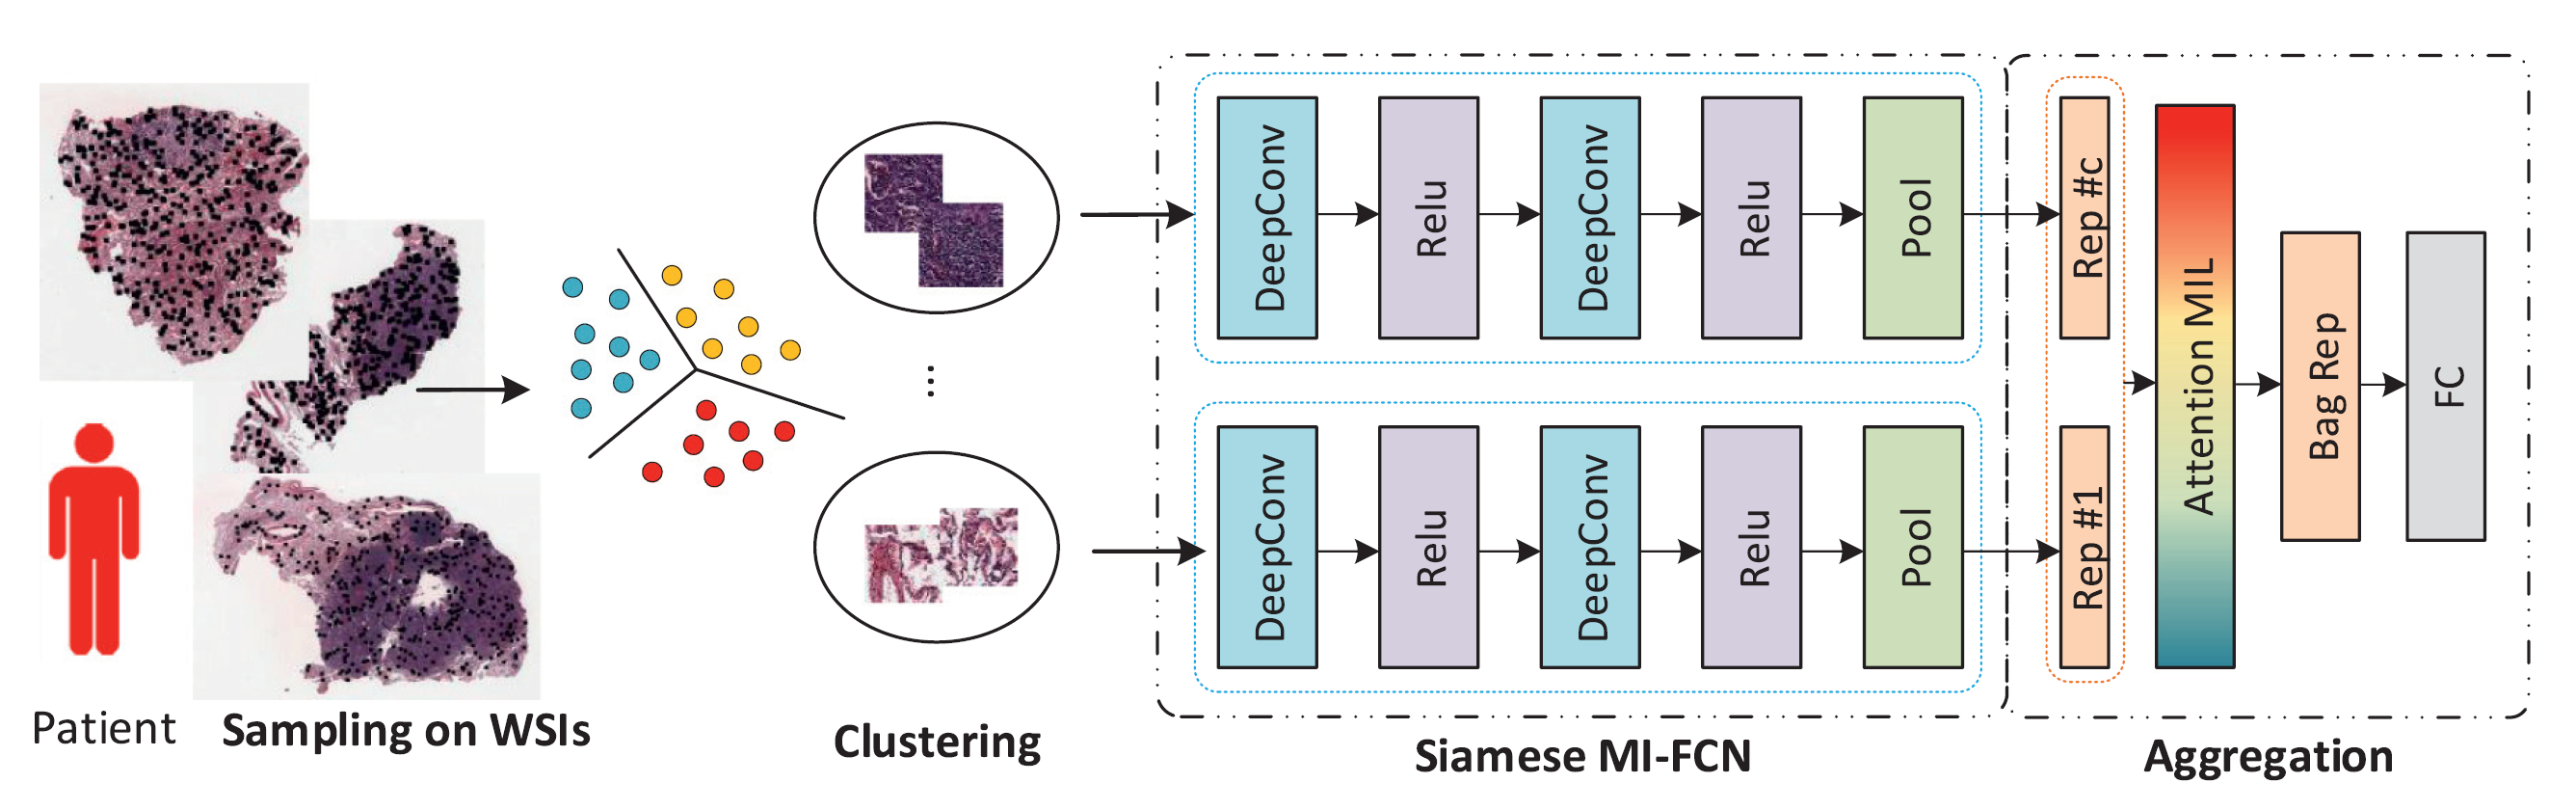
\includegraphics[scale=0.12]{figures/full.png}
			\caption{Overall structure of the proposed framework.}
			\label{fig:full}
		\end{figure}
	\end{frame}
	
	\begin{frame}
		\frametitle{DeepAttnMISL}
		Contributions (cont.) 
		
		\begin{figure}[H]
			\centering
			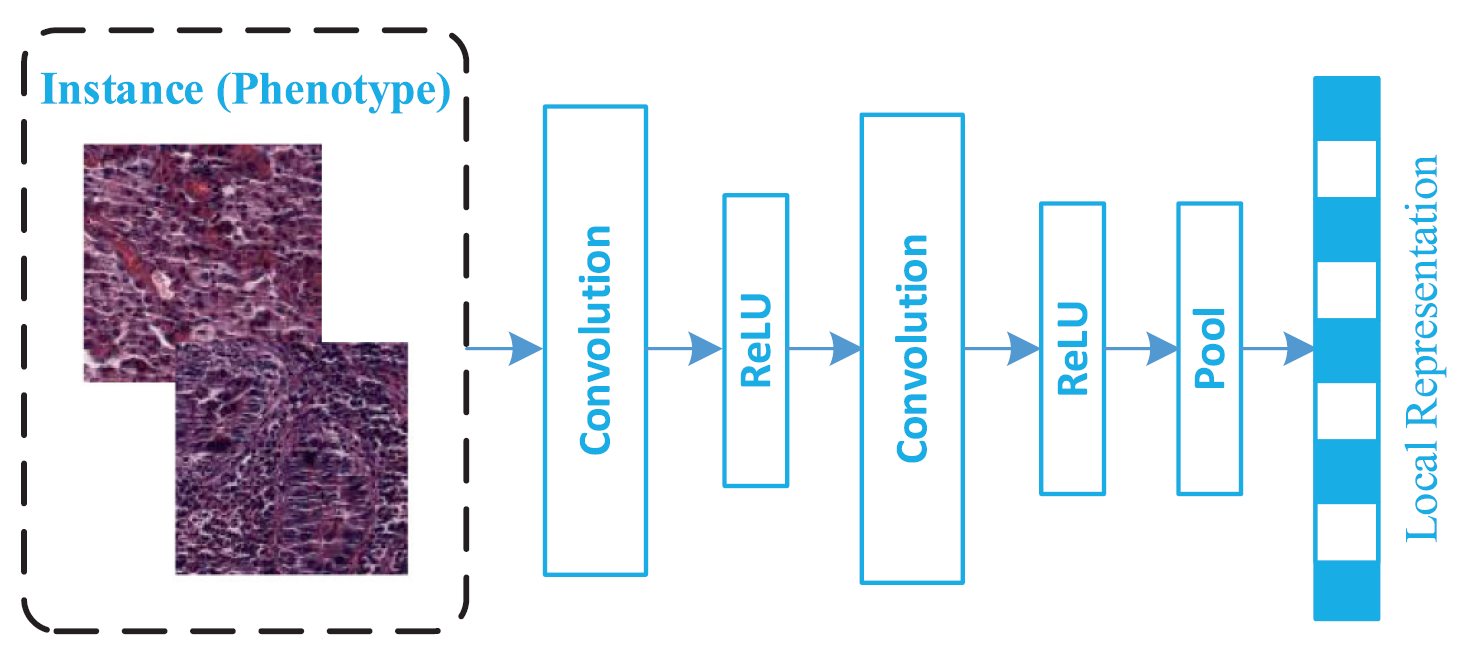
\includegraphics[scale=0.20]{figures/part.png}
			\caption{Structure of each MI-FCN.}
			\label{fig:part}
		\end{figure}
	\end{frame}
	
	\begin{frame}
		\frametitle{DeepAttnMISL}
		Contributions (cont.)
		
		\begin{figure}[H]
			\centering
			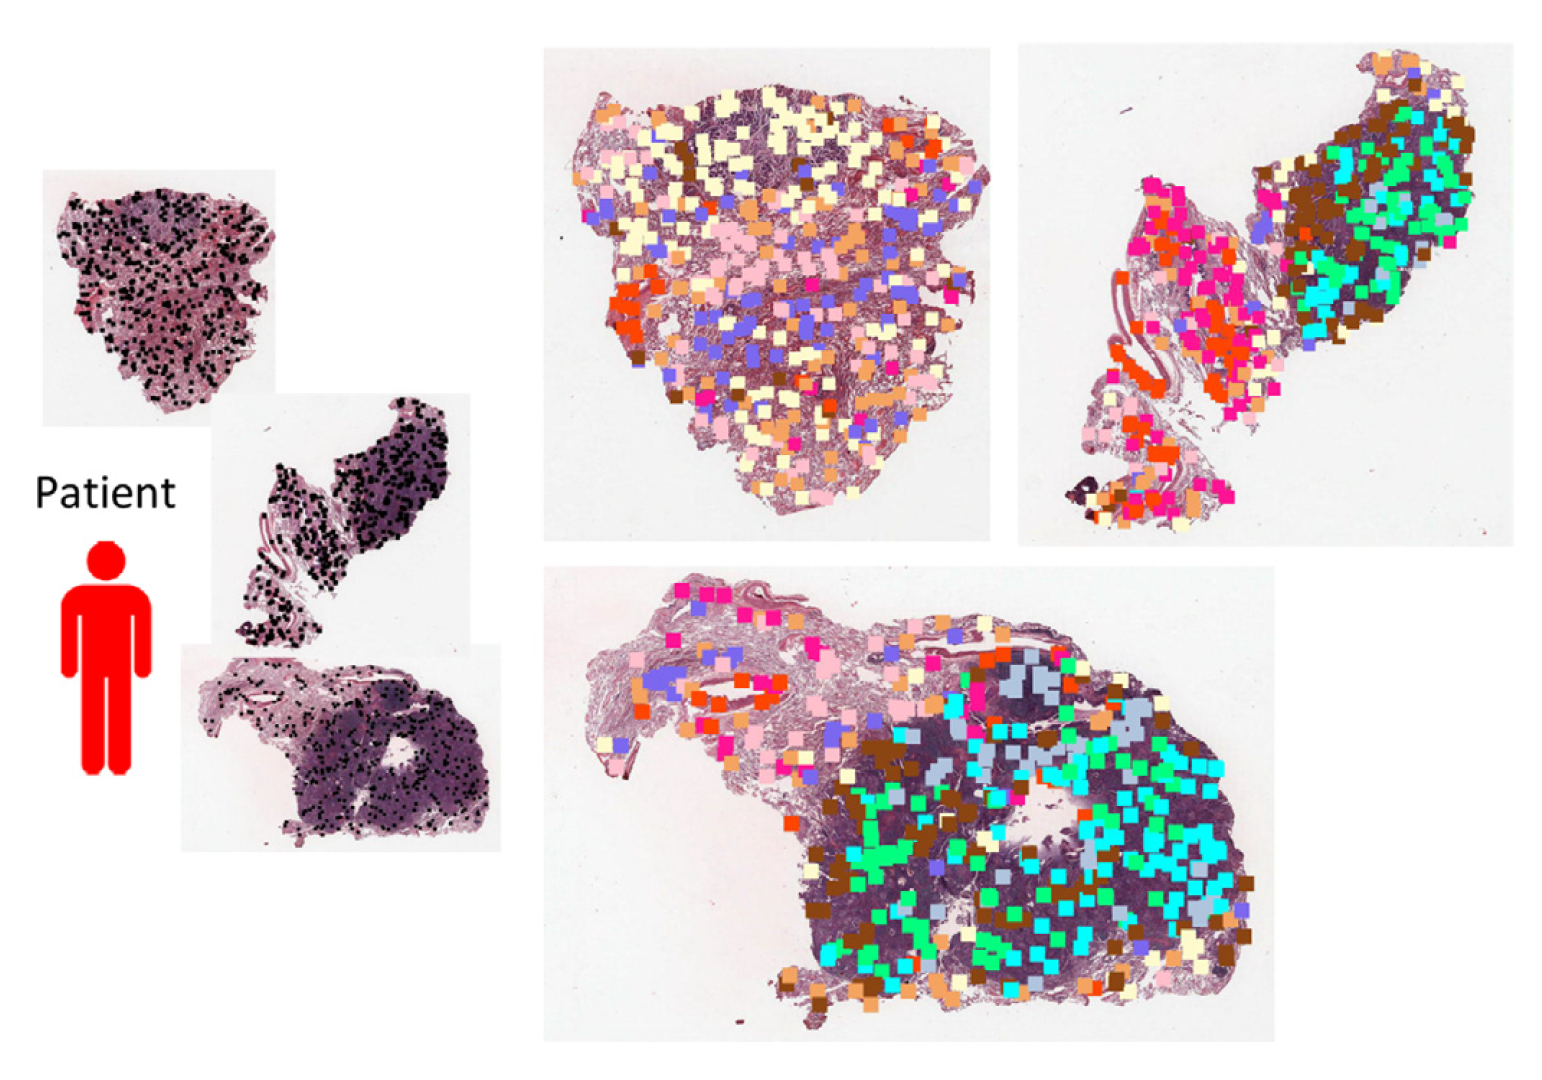
\includegraphics[scale=0.14]{figures/cluster.png}
			\caption{Clustered patches: patches with the same color belong to the same instance.}
			\label{fig:cluster}
		\end{figure}
	\end{frame}

	\begin{frame}
		\frametitle{DeepAttnMISL}
		Contributions (cont.)
		
		\begin{table}[H]
			\begin{center}
				\begin{tabular}{ | l | r | r | r | }
					\hline
					& NLST & MCO\_130K & MCO\_1M \\
					\hline
					Patients & 387 & 1146 & 1146 \\
					\hline
					WSIs & 1177 & 1614 & 1614 \\
					\hline
					Patches & 275244 & 132910 & 915324 \\
					\hline
					Patches/WSI & 234 & 82 & 567 \\
					\hline
				\end{tabular}
			\end{center}
			\caption{The numbers of patients, WSIs, patches and the average number of patches per WSI.}
		\end{table} 
	\end{frame}

	\begin{frame}
		\frametitle{DeepAttnMISL}
		Methodology
		
		\begin{itemize}
			\item Overview \\
			\vspace{5mm}
			Suppose there is a group of patients, $\{ X_i \}, i = 1, \dots, N$ and each of them has a follow-up label $( t_i, \delta_i )$. When $\delta_i = 1$ then $t_i$ is uncensored survival time or failure time, otherwise, $t_i$ is censored survival time.
			
			When dealing with the prognosis problem using multiple instance learning (MIL), a patient is regarded as a bag of instances that $X = \{ x_1, x_2, \dots, x_C \}$, where $C$ denotes the number of instances and may be different for different patients. On the other hand, each instance is a set of patches sampled from WSIs.
		\end{itemize}
	\end{frame}
	
	\begin{frame}
		\frametitle{DeepAttnMISL}
		Methodology (cont.)
		
		\begin{itemize}
			\item Sampling and clustering \\
			\vspace{5mm}
			For each patient, patches are randomly extracted from the WSIs and then clustered into different instances. The 20X pathology images are used for extraction and the patches are of the size $500 \times 500 \times 3$. Then pre-trained deep learning model, e.g. VGG, from ImageNet is used for extracting features from the patches. After that, the features are used for clustering the patches using $k$-means clustering. In the proposed multiple instance learning framework, each cluster is considered as an instance.
		\end{itemize}
	\end{frame}

	\begin{frame}
		\frametitle{DeepAttnMISL}
		Methodology (cont.)
		
		\begin{itemize}
			\item Siamese MI-FCN \\
			A siamese multiple instance fully convolutional network (MI-FCN) is developed to extract features from the instances. The weights of each MI-FCN are shared among all the MI-FCNs. For the $i$th patient, $m_i$ features are fed into the MI-FCN to get the instance-level feature $\mathbf{ r }_i$.
			\item Aggregation via attention-based MIL pooling layer
			Let $R = \{ \mathbf{ r }_1, \dots, \mathbf{ r }_C \}$ be the set of instance-level features. Then patient-level feature is aggregated based on the proposed attention mechanism that 
			\[
			\mathbf{ z } = \sum_{ k = 1 }^{ C } a_k \mathbf{ r }_k,
			\] 
			where $a_k = \frac{ \exp \{ \mathbf{ w }^T \tanh( \mathbf{ V }\mathbf{ r }_k^T ) \}}{ \sum_{ j = 1 }^{ C }\exp \{ \mathbf{ w }^T \tanh( \mathbf{ V }\mathbf{ r }_j^T ) }$, and $\mathbf{ w }$ and $\mathbf{V}$ are weights trained in the neural network.
		\end{itemize}
	\end{frame}
	
	\begin{frame}
		\frametitle{DeepAttnMISL}
		Methodology (cont.)
		
		\begin{itemize}
			\item Loss function \\
			\vspace{5mm}
			Partial likelihood function of the Cox proportional hazards model is used as loss function.
		\end{itemize}
	\end{frame}
	
	\begin{frame}
		\frametitle{DeepAttnMISL}
		Experiments
		
		\begin{itemize}
			\item Data description \\
			\vspace{5mm}
			The NLST dataset is a very large
		\end{itemize}
	\end{frame}
	
	\begin{frame}[allowframebreaks]
		\begin{singlespace}
			\interlinepenalty=10000	% prevents bib items from splitting across pages
			\bibliography{prognosis-medical}
			\bibliographystyle{apalike}
		\end{singlespace}
	\end{frame}
	
\end{document} 